\chapter{Natural Language Generation}

\section{Introduzione alla NLG}

\qs{}{Che cose la \fancyglitter{Natural Language Generation} (NLG)?}

\dfn{Natural Language Generation}{
  Il processo di costruire un testo in \newfancyglitter{linguaggio naturale} per adempiere a specifici goal comunicativi.
}

\nt{Il processo inverso all'analisi. È più facile rispetto all'analisi: per esempio non si ha l'ambiguità perché si decide autonomamente come esprimersi. Non ci bastano gli LLM perché mancano di affidibilità.}

\paragraph{Punti critici del NLG:}

\begin{itemize}
  \item \fancyglitter{Scopo Generale:} un sistema automatico per produrre testo in linguaggio naturale, per comunicare alla maggior platea possibile. 
  \item \fancyglitter{Input:} una forma di rappresentazione dell'informazione di qualsiasi origine. 
  \item \fancyglitter{Output:} documenti, spiegazioni, messaggi d'aiuto, etc. 
  \item \fancyglitter{Basi di Conoscenza:} 
    \begin{itemize}
      \item Sul linguaggio. 
      \item Sul dominio.
    \end{itemize}
\end{itemize}

\nt{La NLG è stata trascurata in passato perché più facile e dunque meno interessante.}

\paragraph{I template (sostanzialmente printf):}

\begin{itemize}
  \item Formalizzazione di basso livello. 
  \item Non servono competenze linguistiche. 
  \item Sono veloci. 
  \item Non sono ottimali quando non si ha ben chiaro l'input.
\end{itemize}

\paragraph{NLG:}

\begin{itemize}
  \item Sono mantenibili. 
  \item Migliore qualità. 
  \item Output multilingua.
\end{itemize}

\nt{Ovviamente sono possibili sistemi ibridi.}

\subsection{BabyTalk}

\dfn{BabyTalk}{
  BabyTalk è un sistema NLG a scopo medico che è diretta a varie persone: dottori, infermiere, famiglie.
}

\paragraph{Punti chiave:}

\begin{itemize}
  \item \fancyglitter{Goal:} produrre dati medici per dottori, infermiere e famiglie. 
  \item \fancyglitter{Input:} dati di sensori, records di azioni o osservazioni dell'equipé medica, etc. 
  \item \fancyglitter{Output:} 
    \begin{itemize}
      \item BT45: 45 minuti di dati per i dottori. 
      \item BT-Nurse: 12 ore di dati per le infermiere. 
      \item BT-Family: 24 ore di dati per le famiglie.
    \end{itemize}
\end{itemize}

\begin{figure}[h]
    \centering
    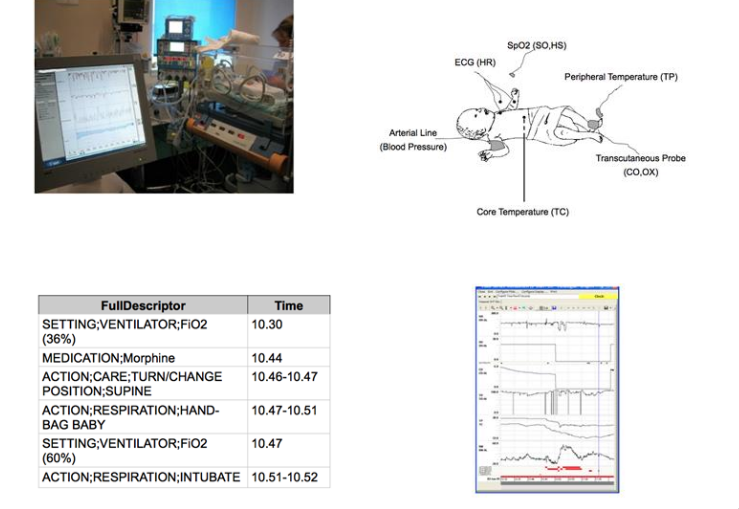
\includegraphics[scale=0.4]{06/bt.png}
    \caption{Esperimento di BabyTalk.}
\end{figure}

\paragraph{Come si è proceduto?}

\begin{itemize}
  \item Si è chiesto a dei dottori di fornire records effettivi per addestrare il sistema. 
  \item Il sistema produce documenti diversi a seconda del destinatario: gli stessi dati possono essere forniti a entrambi, ma con formulazioni diverse (un infermiere capisce un certo tipo di linguaggio mentre un dottore un altro). Stesso per le famiglie.
  \item Si è provato a fare un esperimento con le infermiere: un gruppo con i sensori e l'altro con il testo prodotto da BabyTalk. Quand'è che lavorano meglio?
\end{itemize}

\paragraph{Big Data e NLG:} 

\begin{itemize}
  \item La sempre più grande mole di dati a disposizione ha reso impossibile pensare di leggerli tutti. 
  \item Per cui si sono cominciati ad accorpare NLG e Big Data. 
  \item Inoltre statisticamente i dottori non si fidano del "dato grezzo" (per esempio per interpolazioni, etc.) quindi si va ad utilizzare NLG per spiegare i dati
\end{itemize}

\section{Architetture NLG}

\subsection{I Task della NLG}

\nt{Per gli esempi di questa parte si prenderà in considerazione il dominio dei treni.}

\begin{enumerate}
  \item \fancyglitter{Content determination:} 
    \begin{itemize}
      \item Messaggi provenienti da una struttura dati. 
      \item I messaggi sono aggregazioni di dati che possono essere espressi linguisticamente, con una parola o un sintagma. 
      \item I messaggi sono basati su entità, concetti e relazioni sul dominio. Non c'è nulla di linguistico.  
      \item \evidence{Esempio:} IDENTITY(NEXTTRAIN, CALEDONIANEXPRESS); The next train is the Caledonian Express.
      \item \evidence{Esempio:} DEPARTURETIME(CALEDONIANEXPRESS, 1000); The Caledonian Express leaves at 10am. 
      \item \evidence{Esempio:} COUNT((TRAIN, SOURCE(ABERDEEN),DESTINATION(GLASGOW)), 20, PERDAY); There are 20 trains daily from Aberdeen to Glasgow.
    \end{itemize}
  \item \fancyglitter{Discourse planning:}
    \begin{itemize}
      \item Un testo non è solo un collezione casuale di frasi. 
      \item C'è una struttura che relaziona le frasi. 
      \item Due tipi di relazione:
        \begin{itemize}
          \item Raggrupamento concettuale. 
          \item Relazioni retoriche.
        \end{itemize}
      \item \evidence{Esempio:}
\begin{figure}[h]
    \centering
    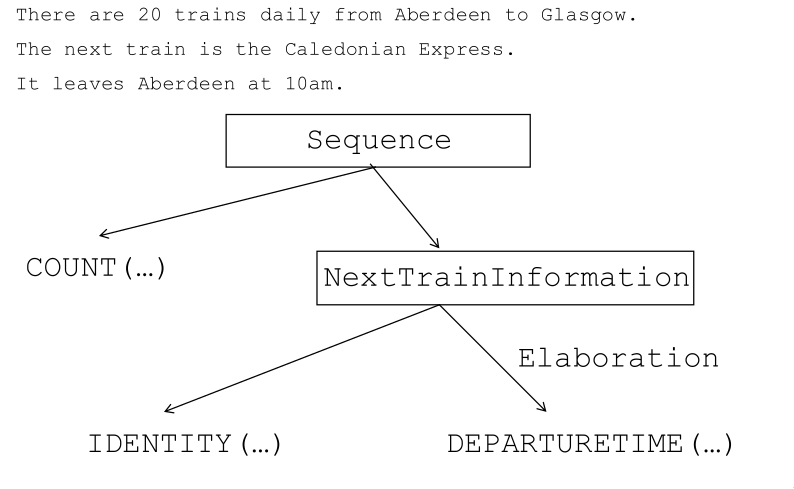
\includegraphics[scale=0.4]{06/dp.png}
\end{figure}

    \end{itemize}
  \item \fancyglitter{Sentence Aggregation:}
    \begin{itemize}
      \item Se si dicessero tutte le frasi 1-a-1 si avrebbe un discorso poco naturale e non fluente. 
      \item Per questo motivo i messaggi vengono combinati per formare frasi più complesse. 
      \item Può causare ambiguità, ma ci si aspetta che l'altro sappia disambiguare.
      \item È il primo task che dipende dalla lingua.
      \item \evidence{Esempio:} The next train, which leaves at 10 am, is the Caledonian Express.
    \end{itemize}
  \item \fancyglitter{Lexicalization:} 
    \begin{itemize}
      \item Determina: 
        \begin{itemize}
          \item Quali parole usare per esprimere i concetti e le relazioni del dominio. 
          \item Quali relazioni sintattiche tra le parole.
        \end{itemize}
      \item \evidence{Esempio:} si deve usare partire o decollare?
    \end{itemize}
  \item \fancyglitter{Referring Expression Generator:}
    \begin{itemize}
      \item Generare le “referrinhg expressions” determina quali parole usare per esprimere le entità del dominio in una maniera comprensibile all'utente. 
      \item Si bilancia fluentazza e ambiguità (a volte con parafrasi).
      \item \evidence{Esempio:} 
        \begin{itemize}
          \item Aberdeen, Scotland. 
          \item Aberdeen.
        \end{itemize}
      \item \evidence{Esempio:}
        \begin{itemize}
          \item The train that leaves at 10am. 
          \item The next train.
        \end{itemize}
    \end{itemize}
  \item \fancyglitter{Syntactic and morphological realization:}
    \begin{itemize}
      \item Ogni lingua ha: 
        \begin{itemize}
          \item Morfologia: come si formano le parole. 
          \item Sintassi: come si formano le frasi.
        \end{itemize}
      \item Arrivati a questo livello il dominio non ha più alcuna importanza, è tutta linguistica.
    \end{itemize}
  \item \fancyglitter{Orthographic realization:} 
    \begin{itemize}
      \item Lettere grandi. 
      \item Punteggiatura. 
      \item Font. 
      \item Impaginazione.
    \end{itemize}
\end{enumerate}










